\section{Clients Control Module}
\label{sec:clients}
This module is used to manage the BGPmon clients. Clients control module consists of a single server thread and multiple client threads.
\begin{itemize}
\item{\emph{Server Thread:} It is a TCP server that listens on a specific port and spawns one client thread for each allowed client. }
\item{\emph{Client Thread:} Each client thread reads the messages from the XML queue and sends them to the client via a TCP connection.}
\end{itemize}
During the initial BGPmon startup, the server thread needs to start first to allow clients to connect before the peering threads begin.  This allows the clients to receive the complete set of messages which is particularly important for logging client.
Some messages will be skipped when a client becomes unresponsive or is unable to keep up with the messages stream. This addresses the need for support of real-time support in BGPmon as slow clients cannot affect the entire system.

\subsection{Data Structure}
The main data structure of clients control module consists of the following fields:
\begin{itemize}
\item{\emph{listenAddr:} The listening socket of server thread binds to this address.  It is a string which could be a IPv4/IPv6 address or one of four keywords(ipv4loopback, ipv4any, ipv6loopback and ipv6any). After it is intialized from configuration, it could be set via command line interface(CLI) at runtime.}
\item{\emph{listenPort:} It is the port on which server thread listens.  It is an integer.  It also could be set via command line interface(CLI) at runtime after initialization.}
\item{\emph{enabled:} It indicates the status of server thread.  If it is false, server thread stops listening but the existing clients still run. Otherwise server thread listens on 'listenPort' and accepts allowed clients. It could be set via CLI  after initialization.}
\item{\emph{maxClients:} It is the max number of clients. It could be set via CLI after initialization. }
\item{\emph{activeClients:} It is the number of connected clients. }
\item{\emph{nextCientID:} It is the ID for the next client to connect. }
\item{\emph{rebindFlag:} If listenAddr or listenPort changes, this flag will be set to TRUE. That means the listening socket of server thread will bind to the new address or port. It is set by CLI.  }
\item{\emph{shutdown:} It is a flag to indicate whether to stop the server thread. }
\item{\emph{lastAction:} It is a timestamp to indicate the last time the thread was active. }
\item{\emph{firstNode:} It is the header of a linked list which maintains the information of all connected clients. Figure \ref{fig:clientsctrl:struct:node} shows the details of client structure of this linked list.}
\item{\emph{clientLock:} It is a pthread mutex lock used to lock the clients info linked list when clients are added or deleted. }
\item{\emph{lastAction:} It is a timestamp to indicate the last time the thread was active. }
This structure is mainly maintained by server thread. 

\subsection{Server Thread}
Server thread has 2 main tasks:
\begin{itemize}
\item{ Listen on "listenAddr" and "listenPort" and periodically every THREAD\_CHECK\_INTERVAL (60s by default) check the values of following three fields. These three fields could be changed by command line interface (CLI).}
	 \begin{itemize}
		\item{\emph{shutdown:} If it is TRUE, the server thread will be closed.}
		\item{\emph{enabled:}  If it is FALSE and "shutdown" is FALSE, close the current listening socket if any.  
									If it is TRUE and "shutdown" is FALSE,  open a new listening socket if there is no listening socket.}			
		\item{\emph{rebindFlag:} If it is TURE and "shutdown" is FALSE, we need to close the current listening socket and open a new listening socket based on the current "listenPort" and "listenAddr".
										This flag is typically set TRUE after changing "listenPort" and "listenAddr". }
		
		\end{itemize}
\item{ Accept the new clients and check them against Access Control List(ACL). }
	 \begin{itemize}
		\item{If a new client pass the ACL check, a new thread will be spawned for it and a new node will be added to the linked list. Then server thread goes back to listen.}
		\item{If a new client doesn't pass the ACL check, the client socket(returned by accept system call) will be close and server thread keeps listening.}
	\end{itemize}	
\end{itemize}

\subsection{Client Thread}
Client thread just reads the messages from XML queue and then writes the messages to the client via socket. Each client thread is associated with the following client structure( See Figure \ref{fig:clientsctrl:struct:node}).
\begin{itemize}
	\item{\emph{id:} identification number of the client. }
	\item{\emph{addr:} client's address. }
	\item{\emph{port:} client's port. }
	\item{\emph{socket:} client's socket for writing messages to the client.}
	\item{\emph{connectedTime:} client's connected time in seconds. }
	\item{\emph{lastAction:} client's last action timestamp. }
	\item{\emph{qReader:} This is a queue reader(see section \ref{sec:queue}). It is used to read messages from XML queue.}
	\item{\emph{deleteClient:} flag to indicate to close the client thread and cleanup client structure.  }
\end{itemize}	
 \begin{figure*}
\centering
\scalebox{1}{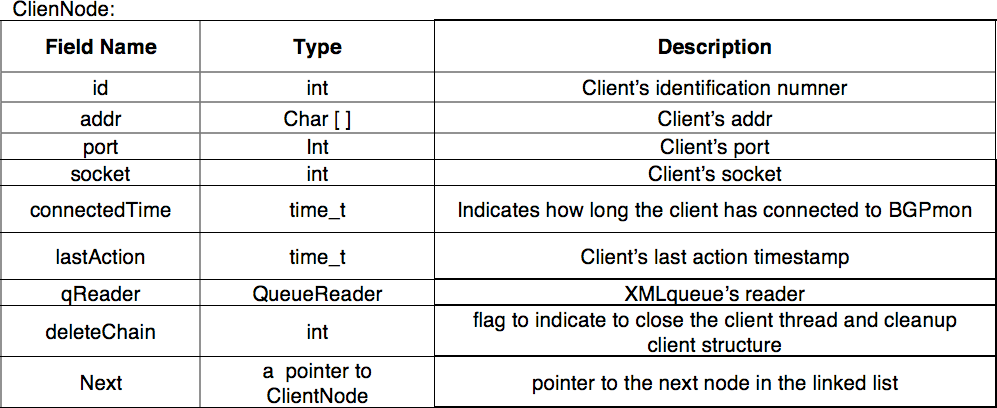
\includegraphics{figs/ClientsctrlNode.pdf}}
\caption{ Client Structure }
\label{fig:clientsctrl:struct:node}
\end{figure*}
\end{itemize}
Note the client thread might exit by itself because of the following 2 reasons:
\begin{itemize}
	\item{ This client thread fails to read the messages from XML queue. In this case, the client thread needs to exit. }
	\item{  This client thread fails to write messages to "socket".}
\end{itemize}
The client thread also might be deleted(call deleteClient) by command line interface(CLI) at running time. Note deleting a client thread is asynchronous action. In other words,  "deleteClient" function only sets the "deleteClient" flag as TRUE. This deletion will be deferred to the next time the child thread checks the "deleteClient" flag. At that time the client thread will exit and the client info in the linked list will be removed. 


\subsection{Design Philosophy}
The important design decision here is that we should let each client specify what they want to receive from BGPmon or we just make BGPmon blindly send everything to the every client.
In the previous design, we did let clients submit their own filters to specify what kind of data they want to receive from BGPmon. But then we realized it would be a huge burden if hundreds of clients all specify their own complex filters.
As our main deign principle is to let BGPmon provide a real-time event stream to a large number of clients, we should relieve BGPmon from the huge burden of handling clients' filters.  As a result, in current design BGPmon simply sends all data to all clients without any processing.  
